% !TEX root       = ./type_name.tex
% !TEX program    = pdflatex
% !TEX encoding   = utf-8
% !TEX spellcheck = de_DE_frami
%=======================================================================

\chapter{Software Defined Networking}\label{ch:software_defined_networking}
\sffamily{}
The Open Network foundation, a non-profit organization, has been undertaking research for the past couple of years in designing and standardizing open network components such as OpenFlow, SDN etc. The Open Network foundation claims that, after the components were rolled out to a variety of network devices and software’s from different vendors. It has been delivering substantial benefits to both enterprises and carriers such as: \cite{What_is_SDN}

\begin{itemize}
	\item \textbf{Directly Programable:}Network directly programmable because the control functions are decoupled from forwarding functions, which enable the network to be programmatically configured by proprietary or open source automation tools.
	\item \textbf{Centralized Management:} Network intelligence is logically centralized in SDN controller software that maintains a global view of the network, which appears to applications and policy engines as a single, logical switch.
	\item \textbf{Reduce CapEx:} Software Defined Networking potentially limits the need to purchase purpose-built, ASIC-based networking hardware, and instead supports pay-as-you-grow models
	\item \textbf{Reduce OpEX:} SDN enables algorithmic control of the network of network elements (such as hardware or software switches/routers that are increasingly programmable, making it easier to design, deploy, manage, and scale networks. The ability to automate provisioning and orchestration optimizes service availability and reliability by reducing overall management time and the chance for human error.
	\item \textbf{Deliver Agility and Flexibility:} Software Defined Networking helps organizations rapidly deploy new applications, services, and infrastructure to quickly meet changing business goals and objectives.
	\item \textbf{Enable Innovation:} SDN enables organizations to create new types of applications, services, and business models that can offer new revenue streams and more value from the network.
	
\end{itemize}
\section{Existing SDN Controllers}\label{existing_sdn_controllers}
For this Master thesis, a few available SDN controllers are first studied for its functionality that can be manipulated for data path segregation. A brief overview on each controller is discussed in the following sections.
\subsection{Ryu Controller \cite{RYU_Switching_Hub}}\label{ryu_controller}
Ryu is a component-based software defined networking framework. It provides software components with well-defined Application Protocol Interfaces (APIs) that make it easy to create new network management and control applications. The component that is of particular interest for this master thesis is the switching hub using OpenFlow.

Switching hubs have a variety of functions like learning the MAC address of the host connected to a port and retaining it in the MAC address table. When receiving packets, the packets that are addressed to a host which is already learned previously is transfered directly to the port connected to the host. Also, when the received packets are addressed to an unknown host, then the switch floods these packets to all ports.



%\begin{itemize}
%	\item Learns the MAC address of the host connected to a port and retains it in the MAC address table.
%	\item When receiving, packets addressed to a host already learned, transfers them to the port connected to the host.
%	\item When receiving, packets addressed to an unknown host, performs flooding.
%\end{itemize}

The main reason to choose RYU over other controllers is due to its customizability and easy to create core applications using Python. RYU allows users to modify core functions or use these functions to create custom applications that suits specific needs, in this case, it was used to create a switching application that can segregate users within the OpenVswitch, instead of being controlled each time by the controller.

The software components provided by RYU with well-defined Application Programming Interface (API’s) as shown in the figure \ref{fig:ryu-controller-sdn-framework}, makes it easy for developers to create custom network management or control applications. The existing components can be quickly and easily be modified or can develop a custom component so that the underlying network can meet the changing demands of the application. RYU is designed to increase the agility of network by being more easily manageable and adapt how traffic is handled.

\begin{figure}
	  \centering
	  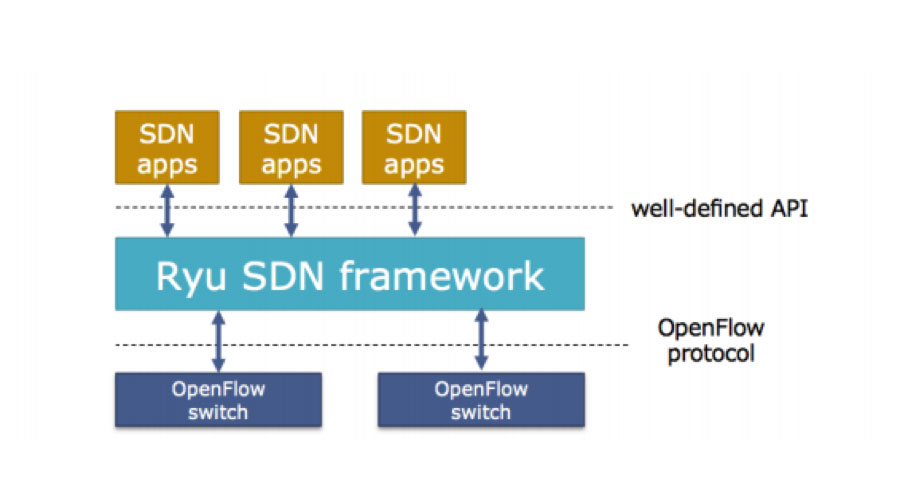
\includegraphics[width=1.0\linewidth]{ryu-controller-sdn-framework}
	  \caption{RYU SDN Controller Framework \cite{ryu_framewrk_png}} \label{fig:ryu-controller-sdn-framework}
	  \vspace{-10pt}
\end{figure}

RYU Controller is supported by the telecommunications company Nippon Telephone and Telegraph (NTT) of Japan and has a strong open source community that maintain and manage the code which is hosted on GitHub. OpenStack, an open source cloud operating system that provides Information as a service (IaaS) \cite{OpenStack} also supports deployment of RYU as network controller in its cloud operating systems.
\subsection{Floodlight Controller \cite{Floodlight_defn}} \label{Floodlight_Controller}

It is yet another open source SDN controller similar to RYU. The benefit of using this controller is its ability to easily develop applications using Java, which is widely used for high level programming by developers and to adapt the software as per requirement. Floodlight offers Representational state transfer application program interfaces (REST APIs) which help developers to easily program interfaces with the product.

Floodlight is used to run as the network backend for OpenStack. When used with the Neutron plugin with OpenStack, the Floodlight controller functions as a network-as-a-service model with the help of REST API offered by Floodlight. The diagram \ref{fig:Floodlight_arch} shows the architecture of Floodlight controller.

\begin{figure}
	\centering
	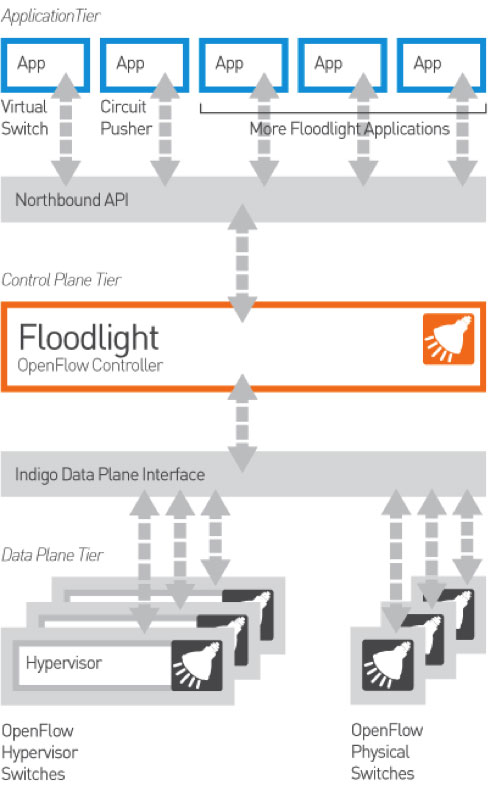
\includegraphics[width=\textwidth, height=\textheight]{floodlight-open-sdn-controller-diagram}
	\caption{Floodlight Controller architecture \cite{Floodlight_arch}} \label{fig:Floodlight_arch}
	\vspace{-10pt}
\end{figure}

The architecture consist of three tiers. The Application tier consist of aplications that work with the controller such as OpenStack, circuit pusher etc. The Control Plane tier is the core of the controller where Floodlight resides, it manages the applications and the switches using OpenFlow. The Northbound APIs also known as REST APIs are used for efficient management of communication between the Floodlight controller and the services and applications running on the network. The Data Plane tier consist of switches such as the Hypervisor (Virtual Switch used by virtual machines) and physical switches. The Indigo Data Plane interface is a software developed by Floodlight that make switch hardware OpenFlow compatible.

\subsection{OpenDaylight} \label{Opendaylight}
OpenDaylight controller is based on JVM, similar to Floodlight, which was a derivative of OpenDaylight that can be deployed on any systems that supports Java. OpenDaylight controller uses the following tools as its framework:

\begin{itemize}
	\item \textbf{Maven:} OpenDaylight uses Maven, which uses Project Object Model to script the dependencies between the bundles for easier build automation.
	\item \textbf{OSGi:} It works as the back-end for OpenDaylight as it loads bundles dynamically and packages JAR files and binding them together for exchange of information.
	\item \textbf{JAVA interfaces:} They are used for event listening, specifications, and forming patterns. 
	\item \textbf{REST APIs:} These are the northbound APIs that manage the topology, flow program, host tracking, static routing and so on.
	
\end{itemize}

The figure \ref{fig:OpenDaylight_framework} shows the framework of OpenDaylight with the above tools mentioned.

\begin{figure}
	\centering
	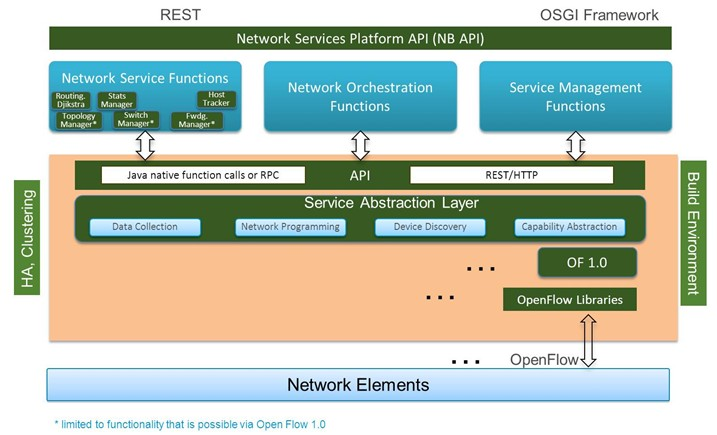
\includegraphics[width=1.0\linewidth]{Architectural_Framework}
	\caption{OpenDaylight Architecture Framework \cite{OpenDaylight_framework}} \label{fig:OpenDaylight_framework}
	\vspace{-10pt}
\end{figure}

\section{Applications of SDN} \label{SDN_applications}

Many research efforts have been conducted until now in writing SDN applications. Jose et. al. \cite{jose2011online} propose using commodity OpenFlow enabled switches for traffic measurement. The authors propose a framework where a collection of rules are installed on OpenFlow switches, and having a controller track the corresponding flow match counters. The controller can then draw inferences from the counters and dynamically tune the rules as required in order to identify different traffic aggregates.

\textit{Resonance} \cite{Nayak:2009:RDA:1592681.1592684} is another application that uses programmable switches to enforce access control in the network. The authors try to prove that today’s enterprise networks rely on different combinations of middle boxes, intrusion detection systems, and network configurations in order to enforce access control policies, whilst placing a burden on end-hosts in the system to remain patched and secure. The proposed system uses the SDN approach comprising of programmable switches and a controller, which together implement a network monitoring framework, a policy specification framework, and the ability to trigger specific actions at the switch level.

\textit{OpenSAFE} \cite{ballard2010extensible} is a framework that enables network monitoring using OpenFlow. It addresses the problem of routing traffic for network analysis in a reliable manner without affecting normal traffic. 

\textit{Hedera} \cite{al2010hedera} is an adaptive flow scheduling system for data center networks. The premise for Hedera is that existing IP multipathing techniques used in data centers usually rely on per-flow static hashing, which can lead to under-utilisation of some network paths over time due to hash collisions. The system works by detecting large flows at the edge switches of a data center, and using placement algorithms to find good paths for the flows in the network. Experiments performed using simulations indicate significant improvements over static load balancing techniques. 

In the paper \textit{OpenFlow based server load balancing gone wild} \cite{wang2011openflow}, the authors address the problem of server load balancing using OpenFlow switches. The number of flow entries that can be saved on an OpenFlow switch is much less than the number of unique flows that a switch might need to handle in data center workloads. Thus, micro flow management using per-flow rules is not practical for performing flow distribution between different servers using a switch. The authors take advantage of OpenFlow’s wildcard based rules capability, and propose algorithms to compute concise wildcard rules that achieve a specific distribution of traffic.

These are some of the applications that have been written for SDN controllers but none of them address the challenge to dynamically redirect packets in real time, based on different clients and their credentials used for authentication. This thesis proposed to build one such application that can segregate packets coming from different clients in such a way that there is no possible connection between multiple clients associated within the same access point.

\section{Open vSwitch \cite{OpenVswitch_design}} \label{OpenvSwitch}
It is a production quality multilayer virtual switch, designed to enable massive automation through programmatic extension. It also supports standard management interfaces and protocols such as NetFlow, sFlow, CLI, port mirroring, VLANs, LACP etc. In addition to this, it is also designed to support distribution across multiple physical servers similar to VMWare’s vNetwork distributed vswitch. Open vSwitch was developed by the Linux foundation and is licensed under Apache 2.0.

The virtual switch is a software layer that resides in a server that is hosting virtual machines. VM’s and also containers such as Docker have logical and virtual Ethernet ports. These logical ports connect to a virtual switch. The diagram \ref{fig:OVS_Features} shows the features of an Open vSwitch. \cite{WhatisOVS}
\begin{figure}
	\centering
	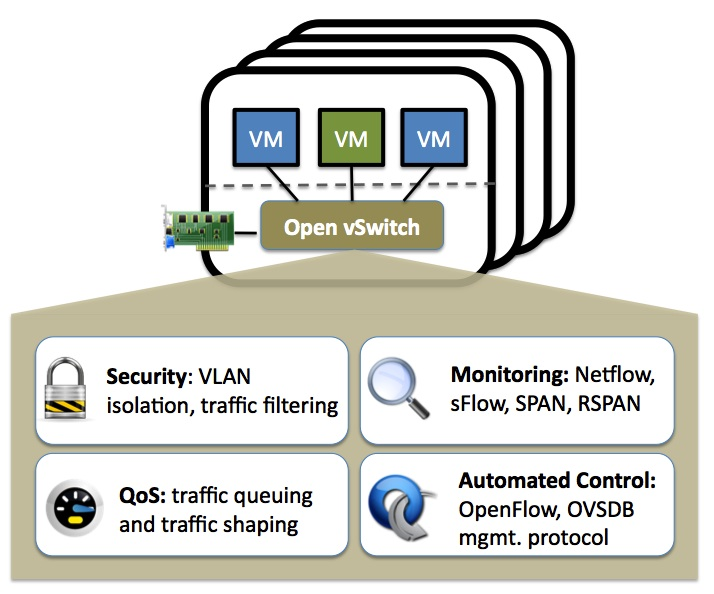
\includegraphics[width=1.0\linewidth]{ovs_schema}
	\caption{Open vSwitch features \cite{ovs_features}} \label{fig:OVS_Features}
	\vspace{-10pt}
\end{figure}

From the management and control perspective, Open vSwitch leverages on the OpenFlow and the Open vSwitch Database (OVSDB) management protocol, which means it can work as both a soft switch running within the hypervisor and as the control stack for switching operations on the physical switches. OVS is also used in SDNs deployed in data centers where it connects all the virtual machines (VMs) within a hypervisor instance on a server. It is the ingress point in overlay networks running on top of the physical networks in the data center and it is the first point of entry for all the VM’s sending traffic to the network. In data center SDN deployments, using OVS for virtual networking is considered the core element since its main use case is a multi-tenant network virtualization. In some service chaining use cases, OVS is sometimes used to direct traffic between network functions.

%\begin{itemize}
%	\item SDN’s deployed in data centers use OVS because it connects all the virtual machines (VMs) within a hypervisor instance on a sever.
%	\item It is the ingress point in overlay networks running on top of the physical networks in the data center and it is the first point of entry for all the VM’s sending traffic to the network.
%	\item In datacenter SDN deployments, using OVS for virtual networking is considered the core element since its main use case is a multi-tenant network virtualization.
%	\item In some service chaining use cases, OVS is sometimes used to direct traffic between network functions.
%	
%\end{itemize}

Open vSwitch is designed in such a way that it is meant to be managed and controlled by third-party controllers and managers. OVS can also directly work with OpenStack using a plugin or directly from an SDN controller, such as OpenDaylight. It is also possible to deploy OVS on all servers in an environment and let it operate with the MAC learning functionality. 